\documentclass[a4paper,twoside,11pt]{article}
\usepackage[english]{babel}
\usepackage[utf8]{inputenc}
\usepackage[T1]{fontenc}
\usepackage{lmodern}
\usepackage[noadjust]{cite}
\usepackage{todonotes}
\usepackage{natbib}
\usepackage{url}
\usepackage{amsmath}
\usepackage{graphicx}
\usepackage{textcomp}
\graphicspath{{images/}}
\usepackage{parskip}
\usepackage{fancyhdr}
\usepackage{vmargin}
\usepackage{tikz}
\usepackage{pstricks}
\usepackage{pst-optexp}
%\usepackage{auto-pst-pdf}
\setmarginsrb{3 cm}{2.5 cm}{3 cm}{2.5 cm}{1 cm}{1.5 cm}{1 cm}{1.5 cm}
%\setmarginsrb{30mm}{20mm}{20mm}{20mm}{0pt}{0mm}{0pt}{0mm}


\usepackage{multicol}
%\usepackage{nonfloat}

%\usepackage{amsfont}
\usepackage{amssymb}

\usepackage[none]{hyphenat}
\usepackage{amsmath}

\usepackage[scientific-notation=true]{siunitx}
\usepackage{subcaption}
%\usepackage[table,xcdraw]{xcolor}
%\usepackage[squaren,Gray]{SIunits}
\usepackage{todonotes}
\usepackage{color}
\usepackage{colortbl}
\usepackage{diagbox}
\usepackage{multirow}
\usepackage{glossaries}
\makeglossaries
\input{glossaire.gls}

\pagestyle{fancy}
\fancyhead{}
\fancyfoot{}
\fancyhead[LE,RO]{\thepage}
\fancyhead[LO,RE]{\rightmark}

\title{Simulation and characterization of integrated optics beam combiners for astrointerferometry}								% Title
\author{Thomas Poletti}								% Author
\date{\today}											% Date

\makeatletter
\let\thetitle\@title
\let\theauthor\@author
\let\thedate\@date
\makeatother


\renewcommand{\headrulewidth}{0pt}
\renewcommand{\footrulewidth}{0pt}

\graphicspath{ {images/} }

\newcommand\frontmatter{%
    \clearpage
  %\@mainmatterfalse
  \pagenumbering{roman}}

\newcommand\mainmatter{%
    \clearpage
 % \@mainmattertrue
  \pagenumbering{arabic}}

\newcommand\backmatter{%
  \if@openright
    \clearpage
  \else
    \clearpage
  \fi
 % \@mainmatterfalse
   }

   
\usepackage[linktoc=all]{hyperref}
\hypersetup{
    colorlinks,
    citecolor=black,
    filecolor=black,
    linkcolor=black,
    urlcolor=black
}

\usepackage[nottoc]{tocbibind}




\makeglossary

\begin{document}

\listoftodos
%%%%%%%%%%%%%%%%%%%%%%%%%%%%%%%%%%%%%%%%%%%%%%%%%%%%%%%%%%%%%%%%%%%%%%%%%%%%%%%%%%%%%%%%%

\begin{titlepage}

	\begin{minipage}{0.5\textwidth}
		\begin{flushleft} 
    %\vspace*{0.5 cm}
    
\includegraphics[scale = 0.6]{phelma.png}\\[1.0 cm]	% University Logo
			\end{flushleft}
			\end{minipage}~
			\begin{minipage}{0.5\textwidth}
            
			\begin{flushright} 
    
    %\vspace*{0.5 cm}
    
\includegraphics[scale = .9]{university.png}\\[1.0 cm]	% University Logo
		\end{flushright}
        
	\end{minipage}\\[3 cm]
	
    \centering
    \vspace*{0.5 cm}
	\rule{\linewidth}{0.2 mm} \\[0.4 cm]
	{ \huge \bfseries \thetitle}\\
	\rule{\linewidth}{0.2 mm} \\[1.5 cm]
    \textsc{\Large I. Physikalisches Institut \\
Universität zu Köln}\\[5 cm]	% University Name
	%\textsc{\Large Grenoble INP-Phelma}\\[0.5 cm]				% Course Code

	
	\begin{minipage}{0.4\textwidth}
		\begin{flushleft} \large
			\emph{Author :} \\
			Thomas Poletti\\
  %           13103057\\
          M1 Physics and NanoSciences\\
          School-year 2017-2018\\
   %         Semester\\
			\end{flushleft}
			\end{minipage}~
			\begin{minipage}{0.4\textwidth}
            
			\begin{flushright} \large
   			\emph{Supervisor:}\\
			Pr. Dr. Lucas Labadie\\
            labadie@ph1.uni-koeln.de\\
		\end{flushright}
        
	\end{minipage}\\[2 cm]
	
    
    
	
\end{titlepage}

\frontmatter
\begin{abstract}
   abstract-text
\end{abstract}
\renewcommand{\abstractname}{Résumé}
\begin{abstract}
   Résumé ici
\end{abstract}
\renewcommand{\abstractname}{Introduction}

\newpage
\tableofcontents
\listoffigures
\listoftables

\clearpage

\mainmatter

\begin{abstract}
Since antiquity and down to our time, astronomers always tried to see further and further in space requiring more and more sensitive instruments. Increasing the telescope diameter is one way to reach higher angular resolution but in the same time make it more sensitive to atmospheric turbulence. Therefore even with the recent progress in adaptative optics, today's largest telescopes can only can only resolve few of the brightest and nearest stars. 

Using individual telescopes to form an interferometer, the resolution is determined by the distance between the telescopes. Until recently the instruments combining the light from individual telescopes were bases on costly and cumbersome bulk optics. The recent advances in manufacturing integrated-optics and especially in laser processing have resulted in new instruments that are operational on sky and delivering higher quality results. 

The purpose of this work is to optimise and characterise the performance of \gls{io} beam combiners and especially one promising type of component called \gls{dbc}. Allowing to retrieve the astronomical parameters without scanning the interferogram these components could allow to observe fast varying objects. 

This report is organised in three parts. In the first part I will present the motivation and the basis of astronomical interferometry. In the second part will be presented the simulation results of the \gls{dbc} as well as its optimisation. In the last part will be discussed the experimental characterisation of asymmetric couplers, \gls{mmi} and of the \gls{dbc}.

\end{abstract}


\section{Motivation and scientific background}

\todo[inline]{- quoi qu’est-ce l’interferometrie, intérêt par rapport à l’observation par un télescope mono-pupille en terme
de résolution angulaire
- Theoreme de VCZ}

\section{Simulation of the DBC}
    
    The discrete beam combiner is a component made of multiple straight waveguides close to each other. It has been demonstrated that in the case of a $N$ telescope \gls{dbc}, an array of more than $N^2$ waveguides is needed for efficient operation of the \gls{dbc} \cite{minardi1}. But at this point is hasn't been studied the impact of other geometrical parameters such as the spacing between each waveguides. 
    
    The component studied is formed of 23 outputs and four inputs to combine the light from four individual telescopes. A cross-section of it is shown on Fig. \ref{tikz:ZigZagCrossSection}. Both the input configuration and the "Zig-Zag" shape have already been optimised. After a brief explanation of the theory behind the \gls{dbc} we will focus on optimising it regarding $P_x$, $P_y$, $width$, $height$ and the length of the \gls{dbc} part (the notations refers to Fig. \ref{tikz:ZigZagCrossSection}) in the case of monochromatic light. In a second part the performances of the optimised component regarding the bandwidth of the input light are simulated. All simulation are performed using the commercial software Beamprop\textcompwordmark{} in scalar mode (a full-vectorial mode would have been more accurate but didn't show much different results for both TE and TM polarisation regarding the condition number of the \gls{V2PM} -see next section-), correlation mode and transparent boundary condition. The grid size was chosen as a balance between computation time and accuracy. The waveguides are simulated by a step-index core.
    \begin{figure}
\resizebox{\textwidth}{!}{
  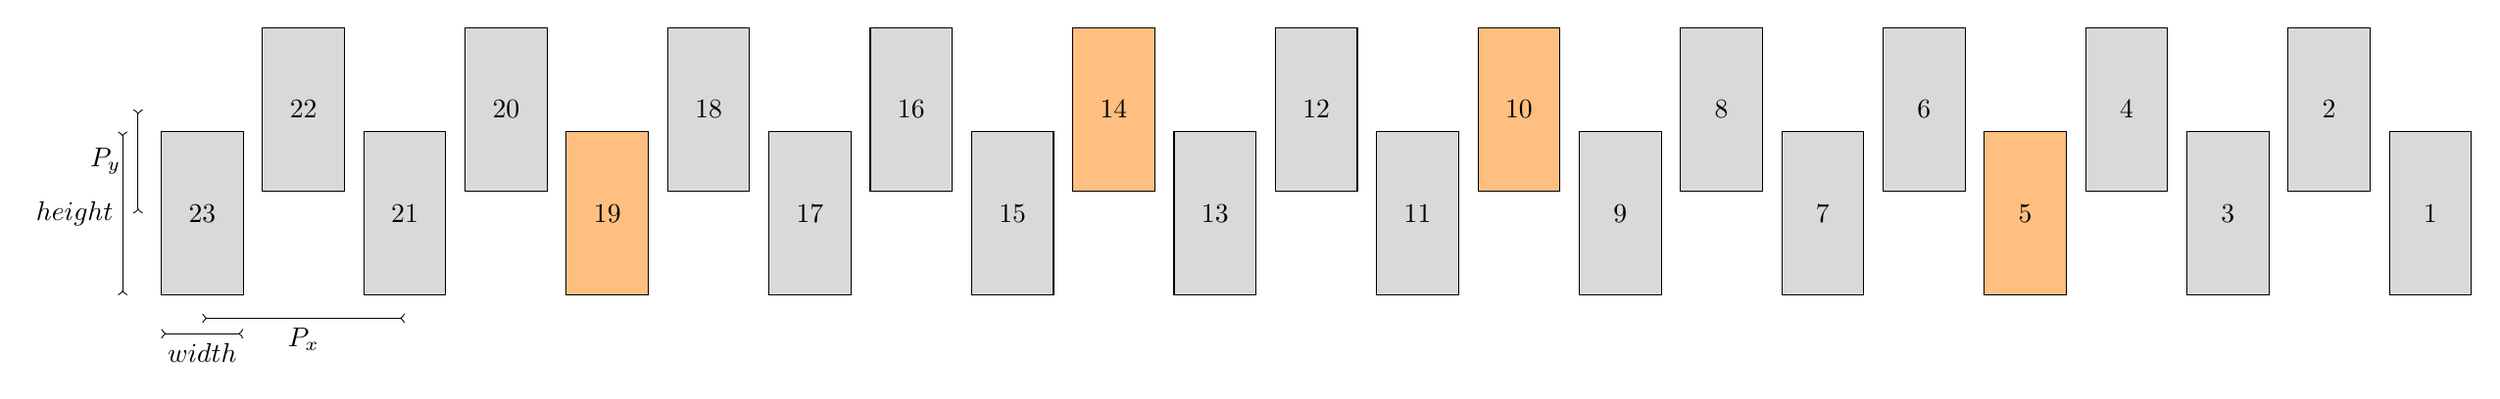
\begin{tikzpicture}

  \def \Px {21/8}
  \def \Py {10.8/8}
  \def \width {8.5/8}
  \def \height {17/8}

  \foreach \i in {0, 1, 2 ,3 ,4 ,5, 6, 7, 8 ,9 ,10, 11}
  {
    \draw[fill=gray!30] (\i * \Px, 0) rectangle (\width + \i * \Px,
    \height);
    \pgfmathtruncatemacro\num{23-2*\i}
    \ifthenelse{\num = 19 \OR \num = 5}{\draw[fill=orange!50] (\i * \Px, 0) rectangle (\width + \i * \Px,
    \height);}{}
    \draw (\width / 2 + \i * \Px, \height / 2) node {\num};
  }

  \foreach \i in {0, 1, 2 ,3 ,4 ,5, 6, 7, 8 ,9 ,10}
  {
   \draw[fill=gray!30] (\Px / 2  + \i * \Px, \Py )
    rectangle (\Px / 2 + \width  + \i * \Px, \Py + \height );
    \pgfmathtruncatemacro\num{22-2*\i}
    \ifthenelse{\num = 14 \OR \num = 10}{\draw[fill=orange!50] (\Px /
      2  + \i * \Px, \Py ) rectangle (\Px / 2 + \width  + \i * \Px, \Py + \height );}{}
    \draw (\width / 2 +\Px / 2 +\i * \Px, \Py + \height / 2) node {\num};
  }

  \draw[>-<] (\width / 2,-.3) -- (\Px + \width / 2,
  -.3);
  \draw (\Px / 2 + \width / 2, -.3) node[below] {$P_x$};
  \draw[>-<] (-.3 , \height / 2) -- (-.3,  \height / 2 + \Py);
  \draw (-.4, \Py /2 + \height / 2) node[left]
  {$P_y$};

  \draw[>-<] (0,-.5 ) -- (\width, -.5);
  \draw (\width / 2, -.5) node[below] {$width$};

  \draw[>-<] (-.5,0) -- (-.5, \height);
  \draw (-.5, \height/2) node[left] {$height$};
\end{tikzpicture}}
\caption{The Zig-Zag array's cross section with the numbering
  convention. The four input waveguides  are displayed in orange.}
\label{tikz:ZigZagCrossSection}

\end{figure}


    \subsection{Monochromatic light}

    In this section is shown the impact on the performances of the \gls{dbc} regarding its geometry. Two main parameters are studied, the condition number of the \gls{V2PM} and the throughput as it hadn't been done before. 
        \subsubsection{Mathematical formalism}\label{sec:mathmono}
         

        
        \subsubsection{Impact of evanescent coupling on the output power}
        
The main principle behind the the \gls{dbc} being the coupling of electromagnetic fields, it is important to understand how much the area chosen to calculate the power at an output could affect the phases relations and visibility. This part focuses on this problem.

Considering  only 3 distinct wave-guides of the DBC Zig-Zag component. The cross section of each WG is a rectangle $width \times height$. In such a dielectric wave-guide, there is no analytical solution to the scalar wave equation but according to \cite{labeye} a good approximation of the transverse field profile is close to a gaussian :
$$
\Psi(x,y) \approx \Psi_0 exp\left( \frac{-x^2}{\omega_x^2} + \frac{-y^2}{\omega_y^2}\right)
$$

Using this equation and retrieving $\omega_x$ and $\omega_y$ from BeamProp simulation by the width of the gaussian at $1/e$ of its maximal amplitude, we can <<calculate>> the transverse field profile in the wave-guide.

We simulate this behaviour for the following parameters (in $\si{\micro\meter}$) :
\begin{itemize}
    \setlength\itemsep{0pt}
\item[-] Px =24
\item[-] Py = 10.8
\item[-] width = 9.5
\item[-] height = 17
\item[-] $n_{clad}$ = 2.31
\item[-] $\delta n$ = 0.005
\end{itemize}
In this case we have $\omega_x \approx 7.798$ and $\omega_y \approx
10.114$. The resulting field for 3 outputs in phase and guiding the same
power is shown in Fig. \ref{fig:3gauss}.

\begin{figure}[htbp]
  \centering
  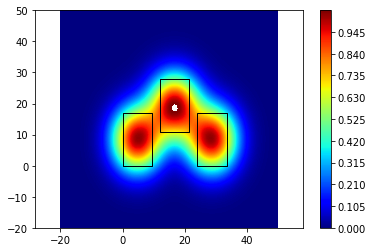
\includegraphics[scale=.5]{picture/integrating_area/3gauss.png}
  \caption{Example of 3 outputs in phase guiding the same power. The modes are Gaussian perfectly centred on the wave-guide}
  \label{fig:3gauss}
\end{figure}

One can see that in this case, where the 3 outputs are in phase, the
determination of the power in the middle WG will be badly estimated by
a simple power integral as : 
\begin{equation} \label{Eq:powerint}
P \propto \iint_{\mathbb{R}^2}
  \Psi^*(x,y)\Psi_{sim}(x,y) dxdy
  \end{equation}
  where $\Psi_{sim}$ is the simulated
output fields as shown on the upper figure. Actually the exact knowledge of the power guided through one individual output is not needed. But if the outputs are not in phase, estimating the "power" by the previous integral would lead to harmonic in the signal vs the \gls{opd}. Therefore the integration
should be limited to a small area around the WG. In the next
paragraph we verify the impact of this choice on the phases
relations, instrumental visibility thus the \gls{V2PM}.

\paragraph{Power of a Gaussian field :}

For an isolated gaussian field the power $P$ is given by \[ \frac{P}{\Psi_0^2} \propto \iint_{\mathbb{R}^2} exp\left( \frac{-2x^2}{\omega_x^2} + \frac{-2y^2}{\omega_y^2} \right) dx dy = \frac{\pi}{2} \omega_x \omega_y\]
In the case of our parameters the right hand is equal to 123.88
$\si{\micro\meter}^2$  (a numerical
integration using the composite trapezoidal rule lead to 123.76). By integrating the whole field as represented
in Fig. \ref{fig:3gauss} over the cross-section we obtain 113.70 $\si{\micro\meter}^2$ but
the truly guided power in the central wave-guide calculated over the
cross-section should only be 87.39 $\si{\micro\meter}^2$ thus an error
of 30 \%. \\
In the opposite case where there is no power in the central
wave-guide, and a maximal power in the two surrounding wave-guides we
find a  guided power in the central wave-guide over the
cross-section of 3.10 $\si{\micro\meter}^2$. It can easily be
understood that the simulated (ergo the experimental) interferograms
will depend of the considered area. The larger this area, the greater the impact of the surrounding wave-guides on the interferogram. In an other hand the smaller this area, the smaller the signal to noise ratio.

\paragraph{Influence on the simulated phases relations :}

We have seen that the integrating area used to estimate the guided
power should have a great
impact on the result, we now try to see its impact on the simulated
phase relations. To do this the 3 gaussian are multiplied by a cosine
to simulate a phase dependency. The left and right outputs are set
with phases pi/3 and 2pi/3 respectively and the middle one with phase
0. The power is then integrated on different area centred on the \gls{wg} cross-section.

One can see that in this case, the phase of the output signal is
mostly unchanged by the integrating area, but this is only the case
for area slightly larger to the WG's cross section. Therefore it
might be expected that the phase relation between outputs with
comparable power magnitude will stay the same for low variation of the
integrating area. The only changed parameter might be the Visibility
but one can not conclude as the mean value, ergo the photometries changes too.

To this point we have only seen the impact of the integrating area when all outputs are guiding the same maximal power. It is now studied the impact on a low guided power in the middle WG
comparatively to the left and right ones. Same phases are
introduced. The power in the left and right WG are the same and 4
times the power in the middle WG. The results to those simulations are
shown in Fig. \ref{fig:phase_influence}
\begin{figure}[htbp]
  \centering
  \begin{minipage}[b]{.33\textwidth}
    \centering
  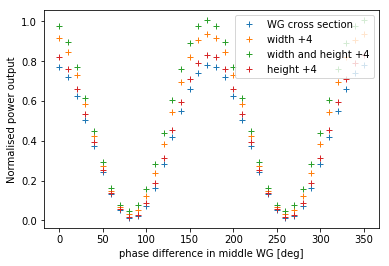
\includegraphics[scale=.35]{picture/integrating_area/phase_python1.png}
    \subcaption{Simulation with the same power in the middle and the surroundings WG.}
  \end{minipage}%
  \hspace{0.2 cm}
  \begin{minipage}[b]{.33\textwidth}
    \centering   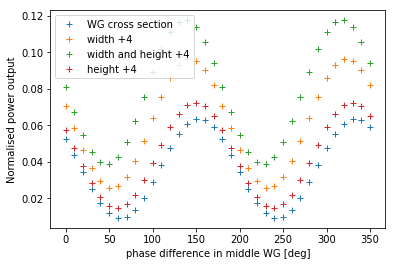
\includegraphics[scale=.35]{picture/integrating_area/phase_python2.png}
    \subcaption{Simulation with low power in the middle WG and high in
    the surroundings.}
  \end{minipage}%
  \hspace{0.2 cm}
  \begin{minipage}[b]{.33\textwidth}
    \centering   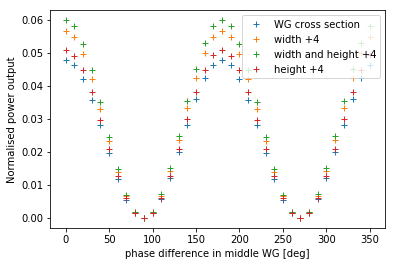
\includegraphics[scale=.35]{picture/integrating_area/phase_python3.png}
    \subcaption{Simulation with low power in the middle WG and high in   \label{fig:forfanout}
    the surroundings for a higher x spacing between the WG.}
  \end{minipage}
  \caption{Influence of different parameters on the phases and
    amplitudes of the interferogram in the middle wave-guide. The phases relations between the outputs are highly influenced by the evanescent coupling}
  \label{fig:phase_influence}
\end{figure}

As can be seen, the more the power difference between the middle WG
and the sides WG and the larger the integrating area, the more
impacted the retrieved phase differences. Therefore it seems that the V2PM matrix of the component should be calculated not only for the isolated component but also with the imaging system. One way to get rid of these dependency would be to have a greater spacing between the WG at the output so that the evanescent coupling is as low as possible (as shown in Fig. \ref{fig:forfanout}). Thus the use of a
<<fan out>> could be an option to calculate the power over a larger area thus have  a greater integrated power
(ergo a smaller signal to noise ratio (SNR)).

        
        \subsubsection{Influence of geometrical parameters}
         

        
       % \subsubsection{Retrieving the visibility function}
       %  

    
    \subsection{Polychromatic light}
    In order to keep a high enough \gls{snr} and also for different needing, the component will be used under poly-chromatic light. In the case of poly-chromatic light, the previous mathematical formalism doesn't hold anymore. In this section will be shown the limitation of the previous formalism, studied the impact of the bandwidth both on the V2MP's condition number and the retrieved mutual coherence function. Experimental results will then be compared to the simulated ones. 
    
        \subsubsection{Mathematical formalism}\label{sec:mathpoly}
        Using polychromatic light, the interferogram at the $n^{th}$ output can be expressed as a function of the optical path difference, x, as follow :
\begin{equation}\label{eq:poly}
In(x) = \int_{-\infty}^{+\infty}I_A(\sigma)\kappa_A(\sigma)+I_B(\sigma)\kappa_B(\sigma)+2\sqrt{I_A(\sigma)\kappa_A(\sigma)I_B(\sigma)\kappa_B(\sigma)}\left| \mu_{AB}(\sigma)\right| cos(\phi_{AB}(\sigma)-2\pi\sigma x) d\sigma
\end{equation}
where $\kappa_i$ relates the transmission from the $i^{th}$ input, $I_i$ the normalized intensity at the $i^{th}$ input, $\left| \mu_{AB}(\sigma)\right| =\left| \mu_{AB}(\sigma)^{inst}\right|\left| \mu_{AB}(\sigma)^{obj}\right| $ the visibility of the interferogram and $\phi_{AB}(\sigma)=\phi_{AB}^{inst}(\sigma)+\phi_{AB}^{obj}(\sigma)$ the phase of the interferogram.
In order to build a V2PM matrix which is independent of the spectrum of the source, it is needed to assume that the spectrum is "flat" within the considered bandwidth. Thus the V2PM matrix will be valid only for quasi-monochromatic light (i.e. a small bandwidth). Doing that the terms $I_i$ are no more wavelength dependant. Eq. \ref{eq:poly} becomes :
\begin{equation}\label{eq:poly2}
In(x) = t_{A}\int_{\sigma}I_Ad\sigma+t_B\int_{\sigma}I_Bd\sigma+2\sqrt{I_AI_B}\int_{\sigma}\sqrt{\kappa_A(\sigma)\kappa_B(\sigma)} \left| \mu_{AB}(\sigma)\right| cos(\phi_{AB}(\sigma)-2\pi\sigma x)d\sigma
\end{equation}
In which $t_i=\frac{\int_{\sigma}I_i(\sigma)\kappa_i(\sigma)}{\int_{\sigma}I_i(\sigma)}$. As our assumption lead us to be limited to quasi-monochromatic light, the visibility should also be relatively independent of the wavelength, as well as the phase if the dispersion of the instrument is negligible. Thus Eq.\ref{eq:poly2} becomes :
\begin{equation}\label{eq:poly3}
In(x) = t_{A}\int_{\sigma}I_Ad\sigma+t_B\int_{\sigma}I_Bd\sigma+2\sqrt{I_AI_B}\left| \mu_{AB} \right|\int_{\sigma}\sqrt{\kappa_A(\sigma)\kappa_B(\sigma)}  cos(\phi_{AB}-2\pi\sigma x)d\sigma
\end{equation}

In order to use the same formalism as in the monochromatic case, we use the so called photocorrection :
$$
\tilde{I_n} = I_n -t_{A}\int_{\sigma}I_Ad\sigma-t_B\int_{\sigma}I_Bd\sigma
$$
\begin{equation}\label{eq:photocorpoly}
V_{AB} =\frac{2\sqrt{I_AI_B}\left| \mu_{AB} \right|\int_{\sigma}\sqrt{\kappa_A(\sigma)\kappa_B(\sigma)}  cos(\phi_{AB}-2\pi\sigma x)d\sigma}{2\sqrt{t_{A}\int_{\sigma}I_A t_B\int_{\sigma}I_B}}
\end{equation}

In that case the visibility function is no longer a cosine, but it can be seen as the Fourier transform of the spectral response of the component (in the case of the a flat spectrum signal used at the input). Thus the visibility function is now something like a cardinal sine, and the narrower the bandwidth, the closest to a cardinal sine it gets.

To use the same V2PM format, the amplitude of visibility is taken at the maximum of this interferogram, where $V_{AB} \approx \left|\mu_{AB}\right|$. The phase is also taken at the position $x_0$ of this maximum and reduced using the formula $\Phi_{AB} \approx 2\pi\sigma_0 x_0$ where $\sigma_0$ is the middle range frequency of the input signal. Taking the nearest point to the "0" OPD is important as will be further explained in the next section.  


        
        \subsubsection{Influence of the bandwidth on the V2PM}
         

        
        \subsubsection{Retrieving the visibility function}
         


\section{Laboratory characterization of the DBC}

    \subsection{characterization setup and method}
    \begin{figure}[htbp!]
 \centering
 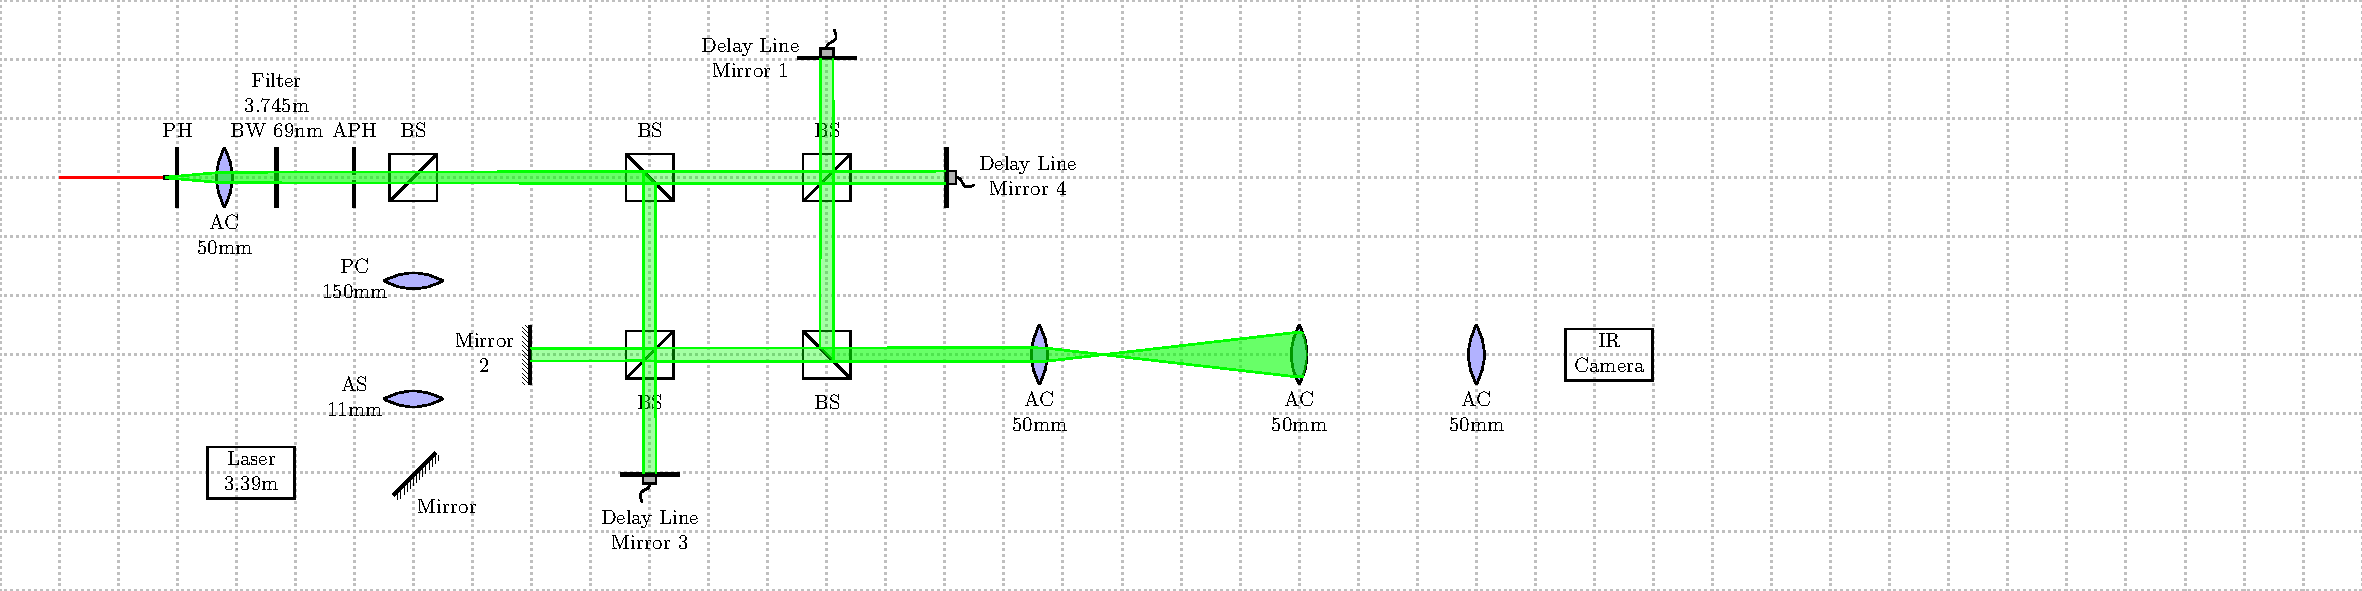
\includegraphics[scale=.53]{../figures/montage.pdf}
 \caption{Experimental setup for characterization of the ZigZag DBC integrated optics chip. The last two lens are used to magnify approximately 8 times. AC = Achromatic, AS = Asphere, PH = PinHole, APH = Adjustable PinHole, BS = Beam-Splitter, PC = Plano-Convex.}
 \label{fig:expersetup}
\end{figure}
 
It has been demonstrated in the previous section that the ZigZag DBC can give accurate results with a bandwidth up to 70nm. The purpose of this part is to verify that experimentally. 
For that purpose the experimental setup represented in Fig.\ref{fig:expersetup} was used. It is a Michelson interferometer with 4 beams. The beams from Mirror 1, 2, 3 and 4 are coupled in the input waveguides 5, 14, 10 and 19 respectively (see Fig \ref{tikz:ZigZagCrossSection} as seen from the input side). 

The DBC used for the characterization is not the one designed in the previous chapter, but is designed to word at 3.4\si{\micro\meter} too. Asit appear that at 3.4\si{\micro\meter} all outputs were not illuminated, the source signal was chosen to be a "flat" spectrum signal of 69nm bandwidth centered at 3.745\si{\micro\meter}. If the component was well inscribed in the glass all photometric signal should be symmetrical (i.e the ones from inputs 2,3 and 4,1 should look alike). As can be seen in Fig.\ref{fig:photometries} this is not the cas especially for inputs 4, 1. The reason of this is to be found in the writing technique. As the laser inscription technique is not the purpose of this report we will simply explain how it induce birefringence. To inscribe the waveguides the laser write multiple lines that overlap each-other. This overlapping lines make the result dependant of the order of inscription of the waveguides which cause the birefringence effect responsible of the not symmetrical pattern. This has to be verified using a polariser.

\begin{figure}
 \centering
 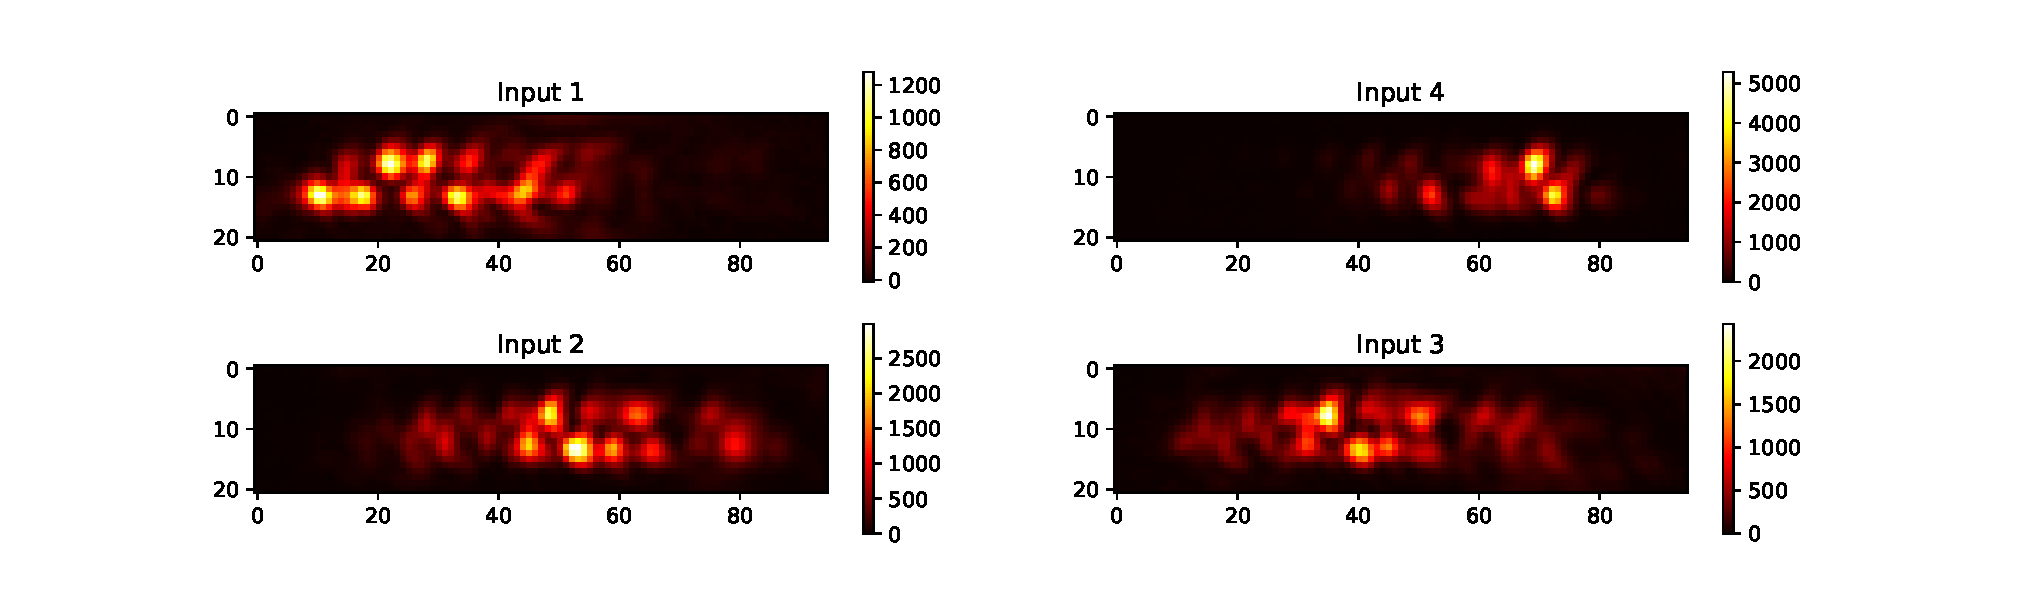
\includegraphics[scale=.45]{photometries.pdf}
 \caption{The photometric signal of the DBC. As can be seen the signal from input 4 ans 1 are not symmetrical certainly due to birefringence.}
 \label{fig:photometries}
\end{figure}

A second point to explain is the presence of the laser. As the Delay-lines were not very accurate in their mouvement, the laser was here to calibrate the OPD. Using the fringe spacing of the laser's interferogram, one can reconstruct the real OPD introduced by the delay-line. In order to do so in a First experiment the laser was coupled into the DBC together with the supercontinum source (at 3.8 \si{\micro\meter}). As it appeared that the laser signal was not enough distinguishable from the source signal this technique was not used to obtain the results presented in the following paragraph.  Rather than doing that, as the "apparent wavelength" of the high-frequency component of the interferogram has been demonstrated to be quite the same for all output at 70nm bandwidth, one interferogram was used to calibrate the OPD stating that the fringe spacing was 3.745\si{\micro\meter}. 

This method is valid in the limit of "apparent frequency" not too different from one output to the other. In fact this was verified as for BL-1/2 the apparent wavelength was $3.75\pm0.05\si{\micro\meter}$, $3.73\pm0.04\si{\micro\meter}$ for BL-1/3, $3.69\pm0.08\si{\micro\meter}$ for BL-1/4, $3.72\pm0.04\si{\micro\meter}$ for BL-2/3, $3.74\pm0.05\si{\micro\meter}$ for BL-2/4 and $3.69\pm0.08\si{\micro\meter}$ for BL-3/4. This is of the same order of magnitude than what was seen in simulation. 

In order to characterize the V2PM, the following measurements are performed for each of the 6 baselines (recording frequency = 100Hz, delay line velocity = 0.08 mm/s):
\begin{enumerate}
 \item Record the signal from the moving delay-line alone $I_{DL}$ with the delay-line moving (5000 frames).
 \item Record the photometry from the non-moving input alone $I_{Fix}$.
 \item Record the interferogram (with the 2 beams) $I$
\end{enumerate}

The obtained result is in the form of a cube of frames. In these frames 1 pixel is chosen to be approximately centered on each output in order to be influenced as little as possible by the surroundings waveguides (as explained in the first chapter. This pixel with the magnification system of 8 should be an area of less than $4\times 4 \si{\micro\meter}$ which was too large in simulation but the best doable at 3.8 µm. - In the case of the component with fanout, one would have to integral all the flux by taking an area around the output in order to have high SNR - . Then the data is processed to build the V2PM as follows :


    \subsection{Retrieving the visibility function}
    
    Having experimentally determined the V2PM and inverted it to obtain the P2VM, the object visibility and phase are retrieved from the experimental  data. First using the same set of data used to calibrate the V2PM and then using new ones to test the reproducibility of the method. 

The results of the retrieved phases from the data used to calibrate the V2PM matrix are shown on Fig.\ref{fig:retrieved_visi_expe}. These results aren't biased by the calibration of the V2PM because the V2PM only take into account of the visibility and phase of the output interferogram at the position of their maximum. What is flagrant from these results and the simulated ones on a similar component (see \ref{an:retrieved_visi_simu}) is that experimentally the retrieved visibility tend to oscillate a lot more around the theoretical one (expecially for baseline 14. These oscillations are mostly due to the highly overlapping output signal (as explained in the first chapter) and the delay-line being not verry accurate thus changing the coupling a little from one measurement to the other (this will be verified further). Contributions of the noise are also not negligible. With all of these imperfections the retrieve visibility are around the zone of interest (around the maximum) accurate at 10\% for the best baselines to 20\% for the worst. The visibilities retrieved on the second dataset recorded right after the calibration of the V2PM are presented on figure \ref{fig:retrieved_visi_expe2} and are far from as good as the first ones. This is mostly because of the delay-line altering the coupling in its mouvement.  


\begin{figure}[htbp!]
 \centering
 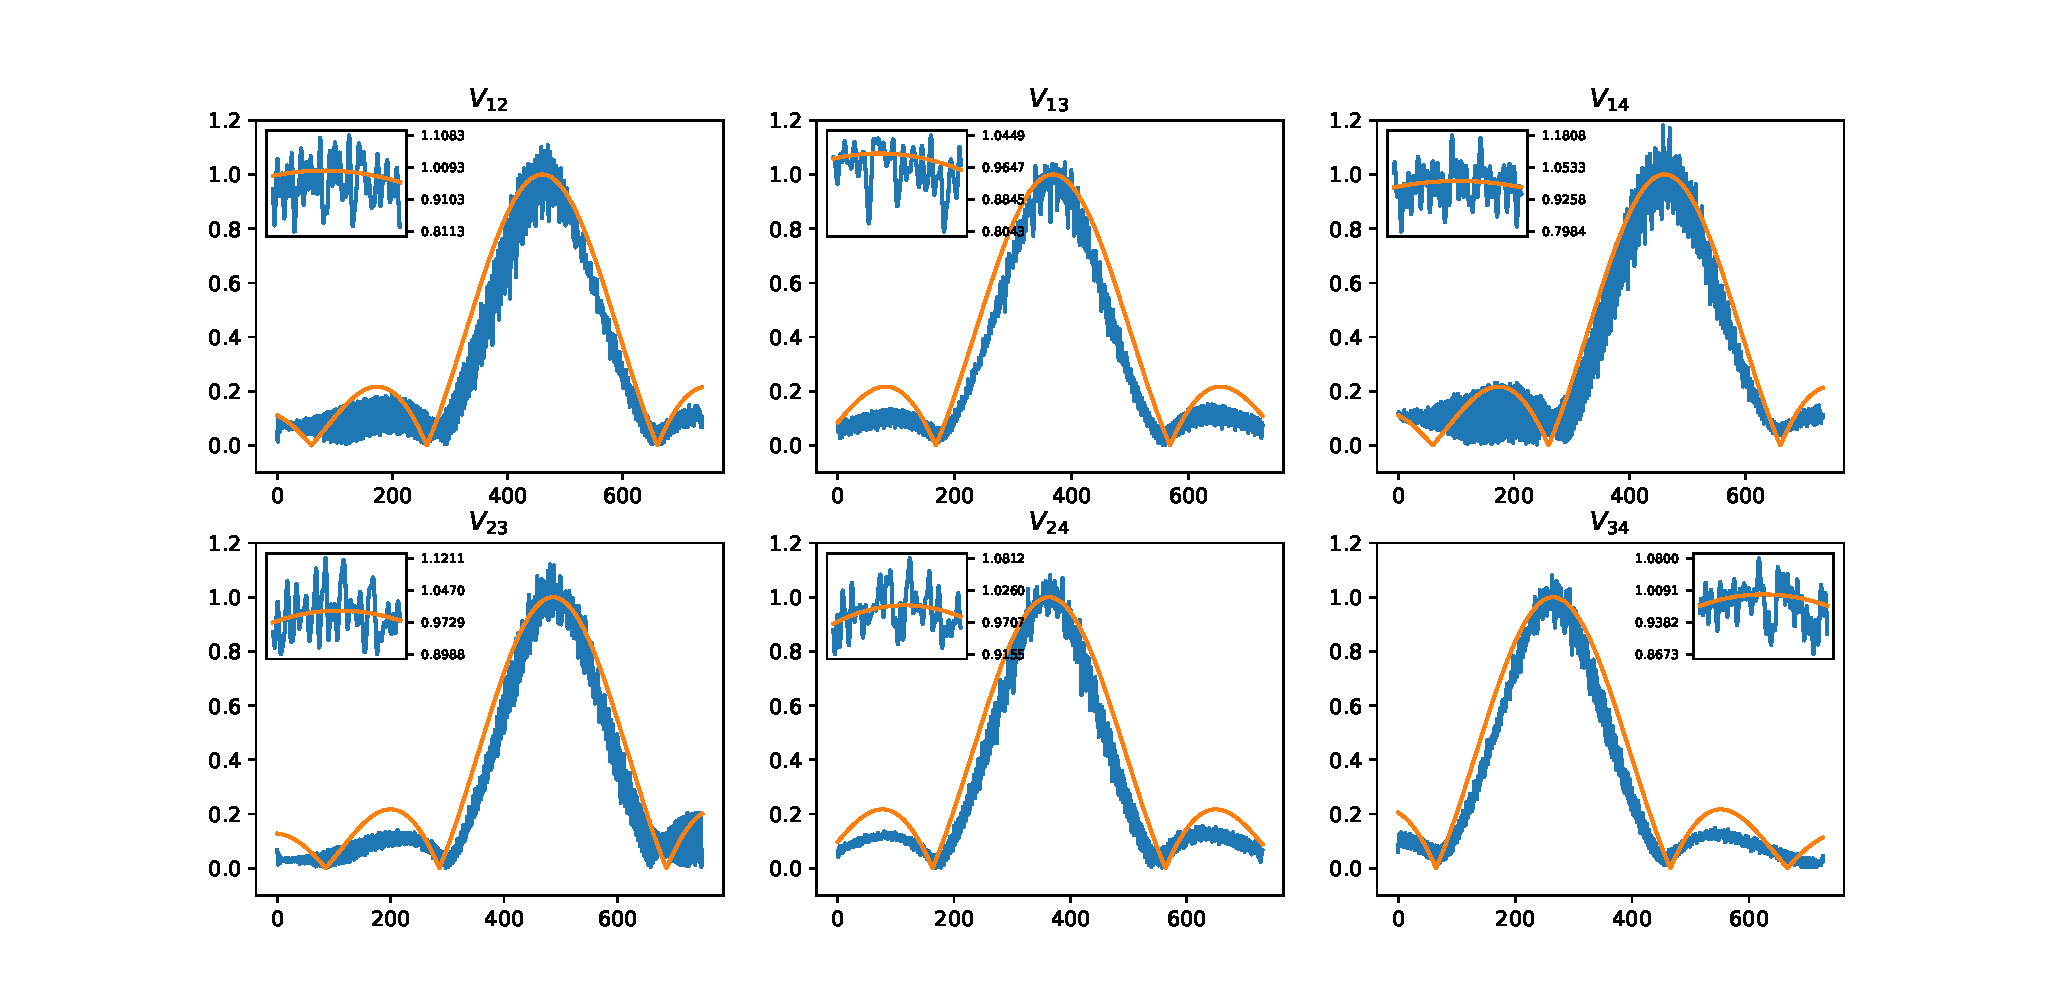
\includegraphics[scale=.45]{../picture/retrieve_visi_expe.pdf}
 \caption{Experimentally retrieved visibility from the dataset used to calibrate the V2PM. Baselines numbering 1, 2, 3, 4 refers to the input waveguides (respectively  9, 14, 10 and 19). The blue line is the actual retrieved data and the orange line the theoretical result. The inset is a zoom of the 50µm opd around the maximum. }
 \label{fig:retrieved_visi_expe}
\end{figure}

\begin{figure}[htbp!]
 \centering
 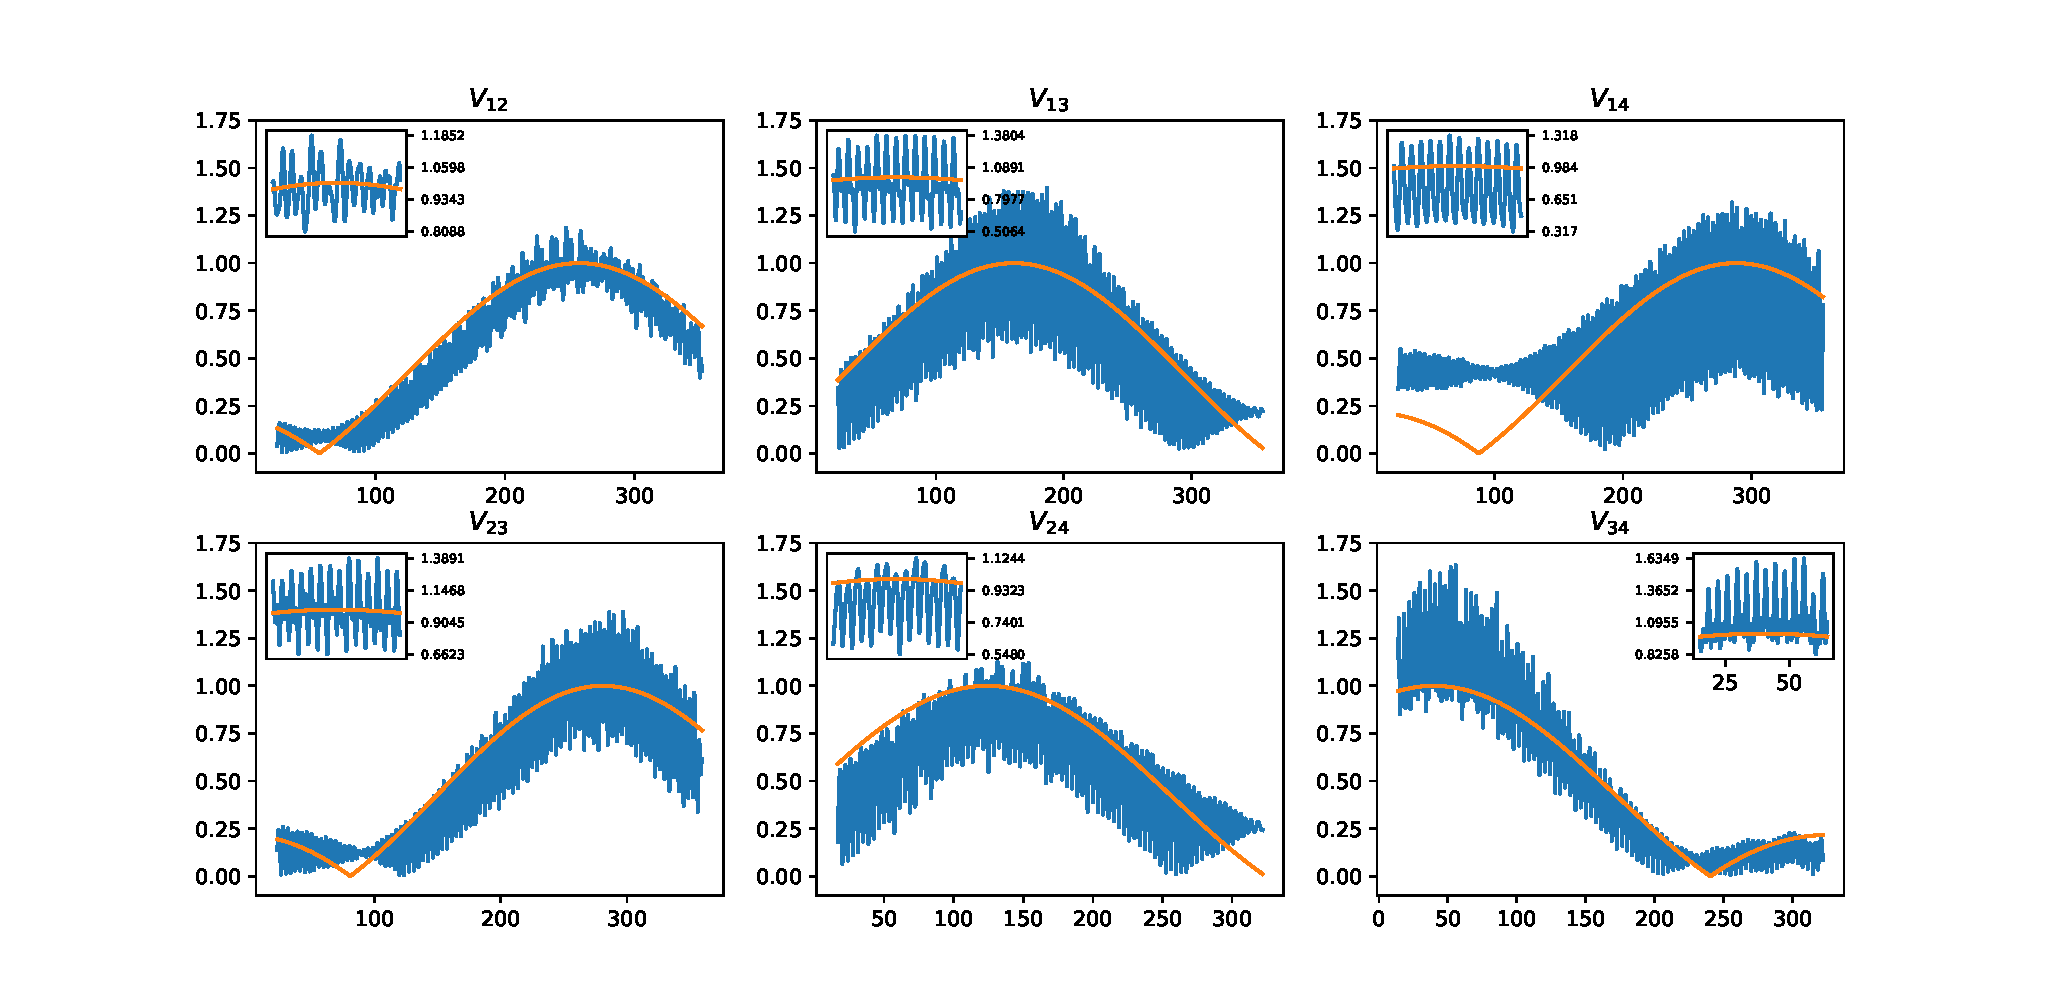
\includegraphics[scale=.45]{../picture/retrieve_visi_expe2.pdf}
 \caption{Experimentally retrieved visibility from the data recorded after the V2PM calibration. Baselines numbering 1, 2, 3, 4 refers to the input waveguides (respectively  9, 14, 10 and 19). The blue line is the actual retrieved data and the orange line the theoretical result. The inset is a zoom of the 50µm opd around the maximum. }
 \label{fig:retrieved_visi_expe2}
\end{figure}

Concerning the retrieved phase, the results are presented in Fig\ref{fig:retrieved_phase_expe} for the dataset used to calibrate the V2PM and Fig.\ref{retrieve_phase_expe2} for the second dataset zoomed around the maximum.

\begin{figure}[htbp!]
 \centering
 \includegraphics[scale=.45]{../picture/retrieve_phase_expe.pdf}
 \caption{Experimentally retrieved phase from the dataset used to calibrate the V2PM. Baselines numbering 1, 2, 3, 4 refers to the input waveguides (respectively  9, 14, 10 and 19). The blue line is the actual retrieved data and the orange line the theoretical result. }
 \label{fig:retrieved_phase_expe}
\end{figure}

\begin{figure}[htbp!]
 \centering
 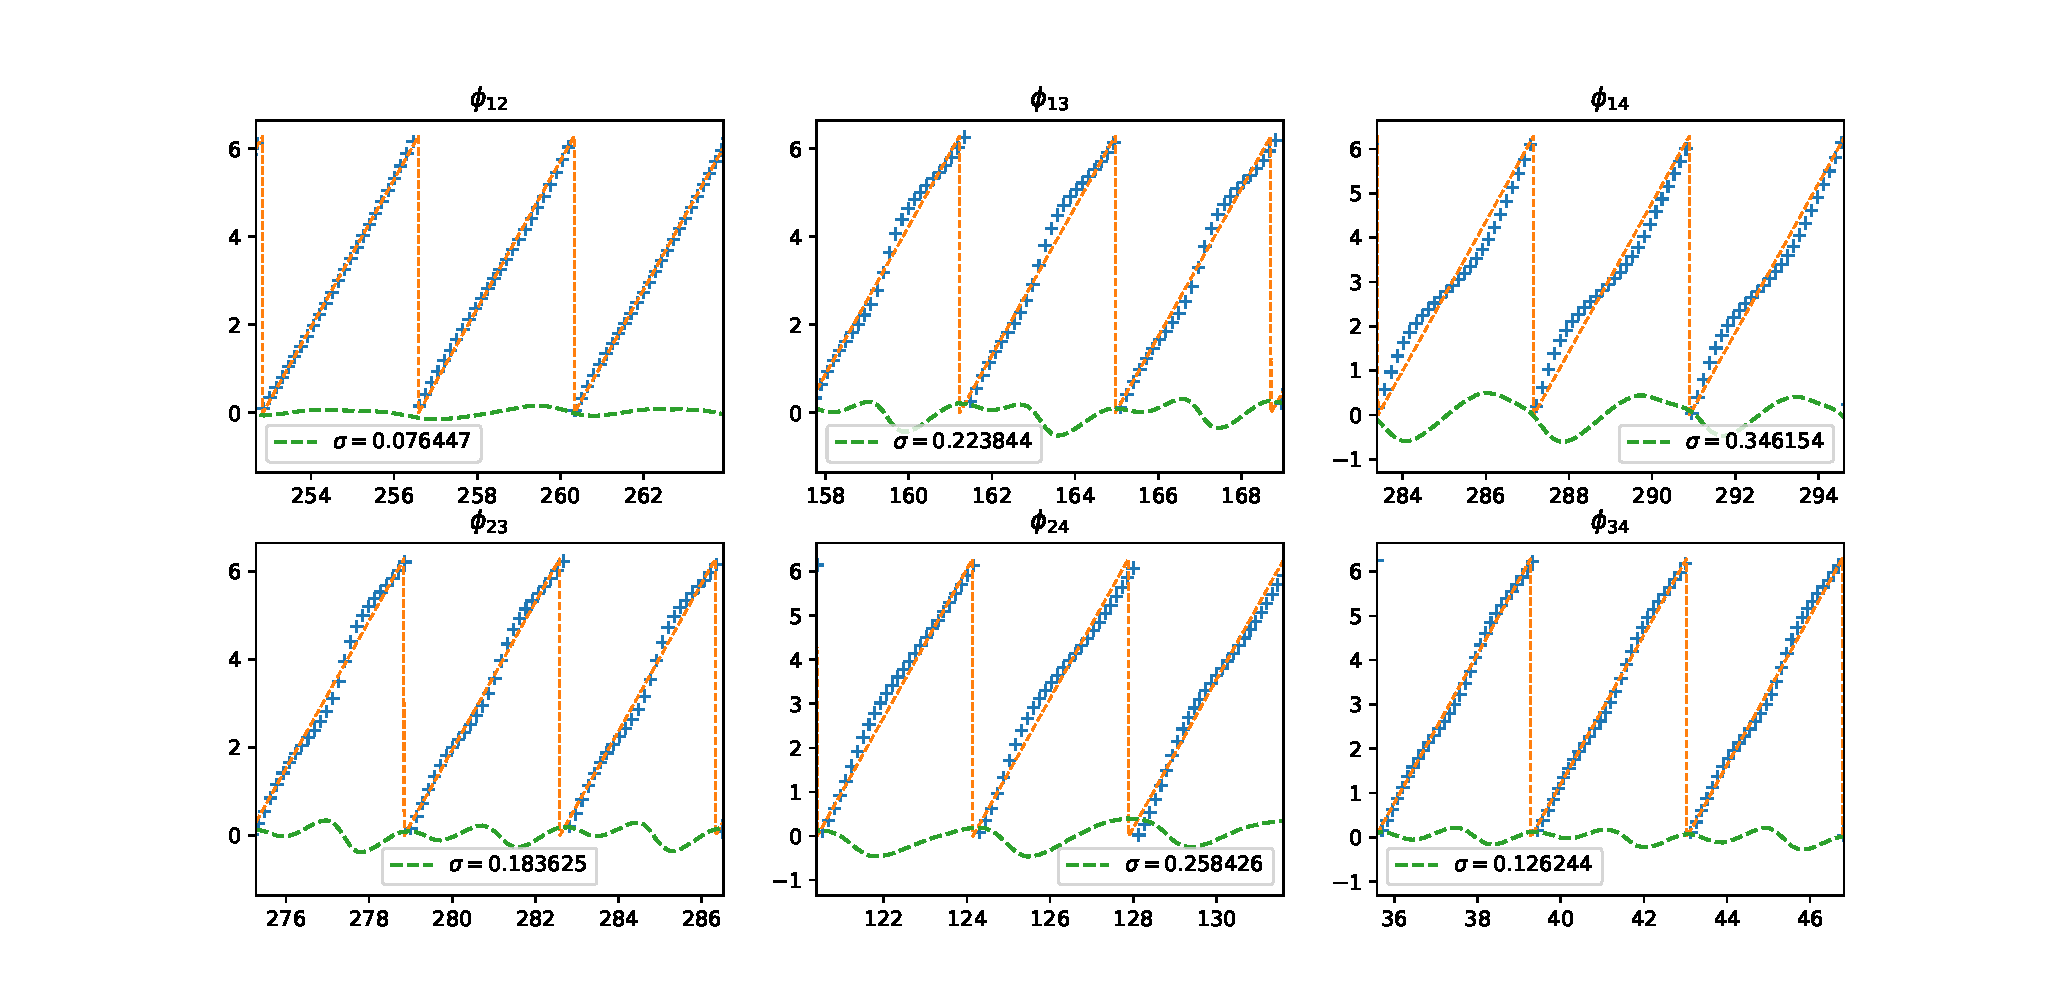
\includegraphics[scale=.45]{../picture/retrieve_phase_expe2.pdf}
 \caption{Experimentally retrieved phase from the data recorded after the V2PM calibration. Baselines numbering 1, 2, 3, 4 refers to the input waveguides (respectively  9, 14, 10 and 19). The blue line is the actual retrieved data and the orange line the theoretical result. }
 \label{fig:retrieved_phase_expe2}
\end{figure}

    
\section*{Conclusion and Further-work}

\backmatter
\appendix
\section{Appendix}
    \subsection{The condition number}\label{an:cond}
    Considering the following system $A\vec{x}=\vec{b}$ where A is the
matrix describing our system (A is a matrix with real coefficients). An error $\vec{\delta x}$ on $\vec{x}$
will lead to an error $\vec{\delta b}$ on $\vec{b}$. The aim is to
know how much bigger or smaller is $\frac{\left\|\vec{\delta x}
  \right\|}{\left\|\vec{x} \right\|}$ compared to $\frac{\left\|\vec{\delta b}
  \right\|}{\left\|\vec{b} \right\|}$ (i.e how much an error is
magnified by the A matrix).

In the case where A in neither symmetric nor square. Then the matrix
$A^TA$ is a square symmetric matrix and Then can be diagonalized. Lets
call $\lambda_i$ and $\vec{u_i}$ its eigenvalues and eigenvectors. We
can write : $$ A^TA \vec{u_i} = \lambda_i \vec{u_i}$$
Moreover $$\left\| A\vec{x}\right\|^2 = \vec{x}^TA^TA\vec{x} =
\left\| \vec{b}\right\|^2$$
So $\left\| \vec{b} \right\|^2 \leq max(|\lambda_i|) \left\| \vec{x}
\right\|^2$ and $\left\| \vec{\delta b} \right\|^2 \geq
min(|\lambda_i|) \left\| \vec{\delta x}
\right\|^2$ and then :
$$\boxed{
\frac{\left\|\vec{\delta x}
  \right\|}{\left\|\vec{x} \right\|} \leq \frac{\sqrt{max(|\lambda_i|)}}{\sqrt{min(|\lambda_i|)}} \frac{\left\|\vec{\delta b}
  \right\|}{\left\|\vec{b} \right\|}
}$$

The number $\frac{\sqrt{max(|\lambda_i|)}}{\sqrt{min(|\lambda_i|)}}$
where $min(|\lambda_i|)$ is the minimal non zero eigenvalue of $A^TA$,
is called the condition number of the A matrix. It means how much an
error on the right part of the system can be magnified by the A matrix.

\newpage
    \subsection{Simulated retrieved Phase and visibility}\label{an:retriev}
    In order to compare the results of Fig.\ref{fig:retrieve_visi_expe} in a more readable way than with Fig.\ref{fig:retrieved_fan} the reader can see the results on the following plot.
    \begin{figure}[htbp!]
     \centering
     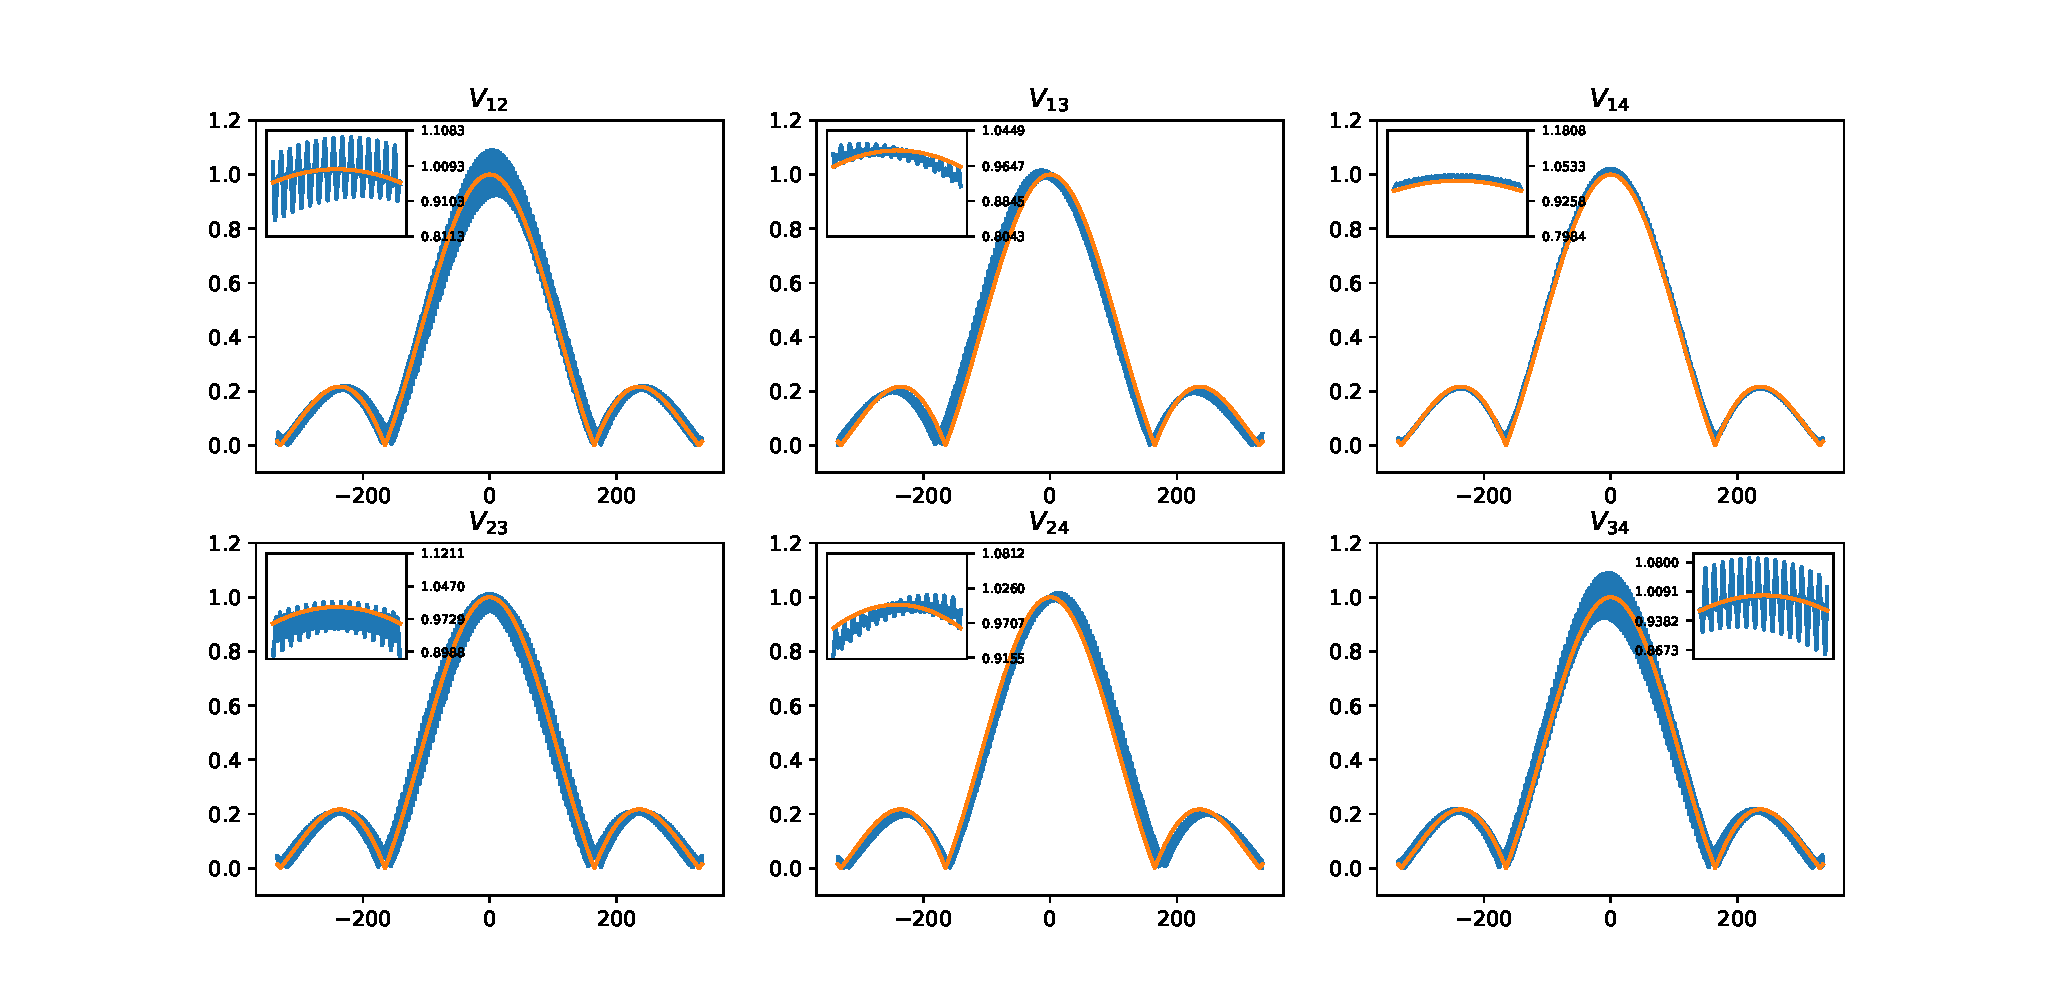
\includegraphics[scale=.4]{../picture/retrieve_visi_simu.pdf}
     \caption{The simulated retrieved visibilities of the optimised component at $\lambda=3.4\si{\micro\meter}$ and bandwidth=70nm. The x-axis is the OPD in µm and the y-axis the visibility. Baseline numbering follows the ones from Fig.\ref{fig:retrieved_visi_expe}.The blue line is the actual retrieved data and the orange line the theoretical result.}
     \label{an:retrieved_visi_simu}
    \end{figure}
    
    \begin{figure}[htbp!]
     \centering
     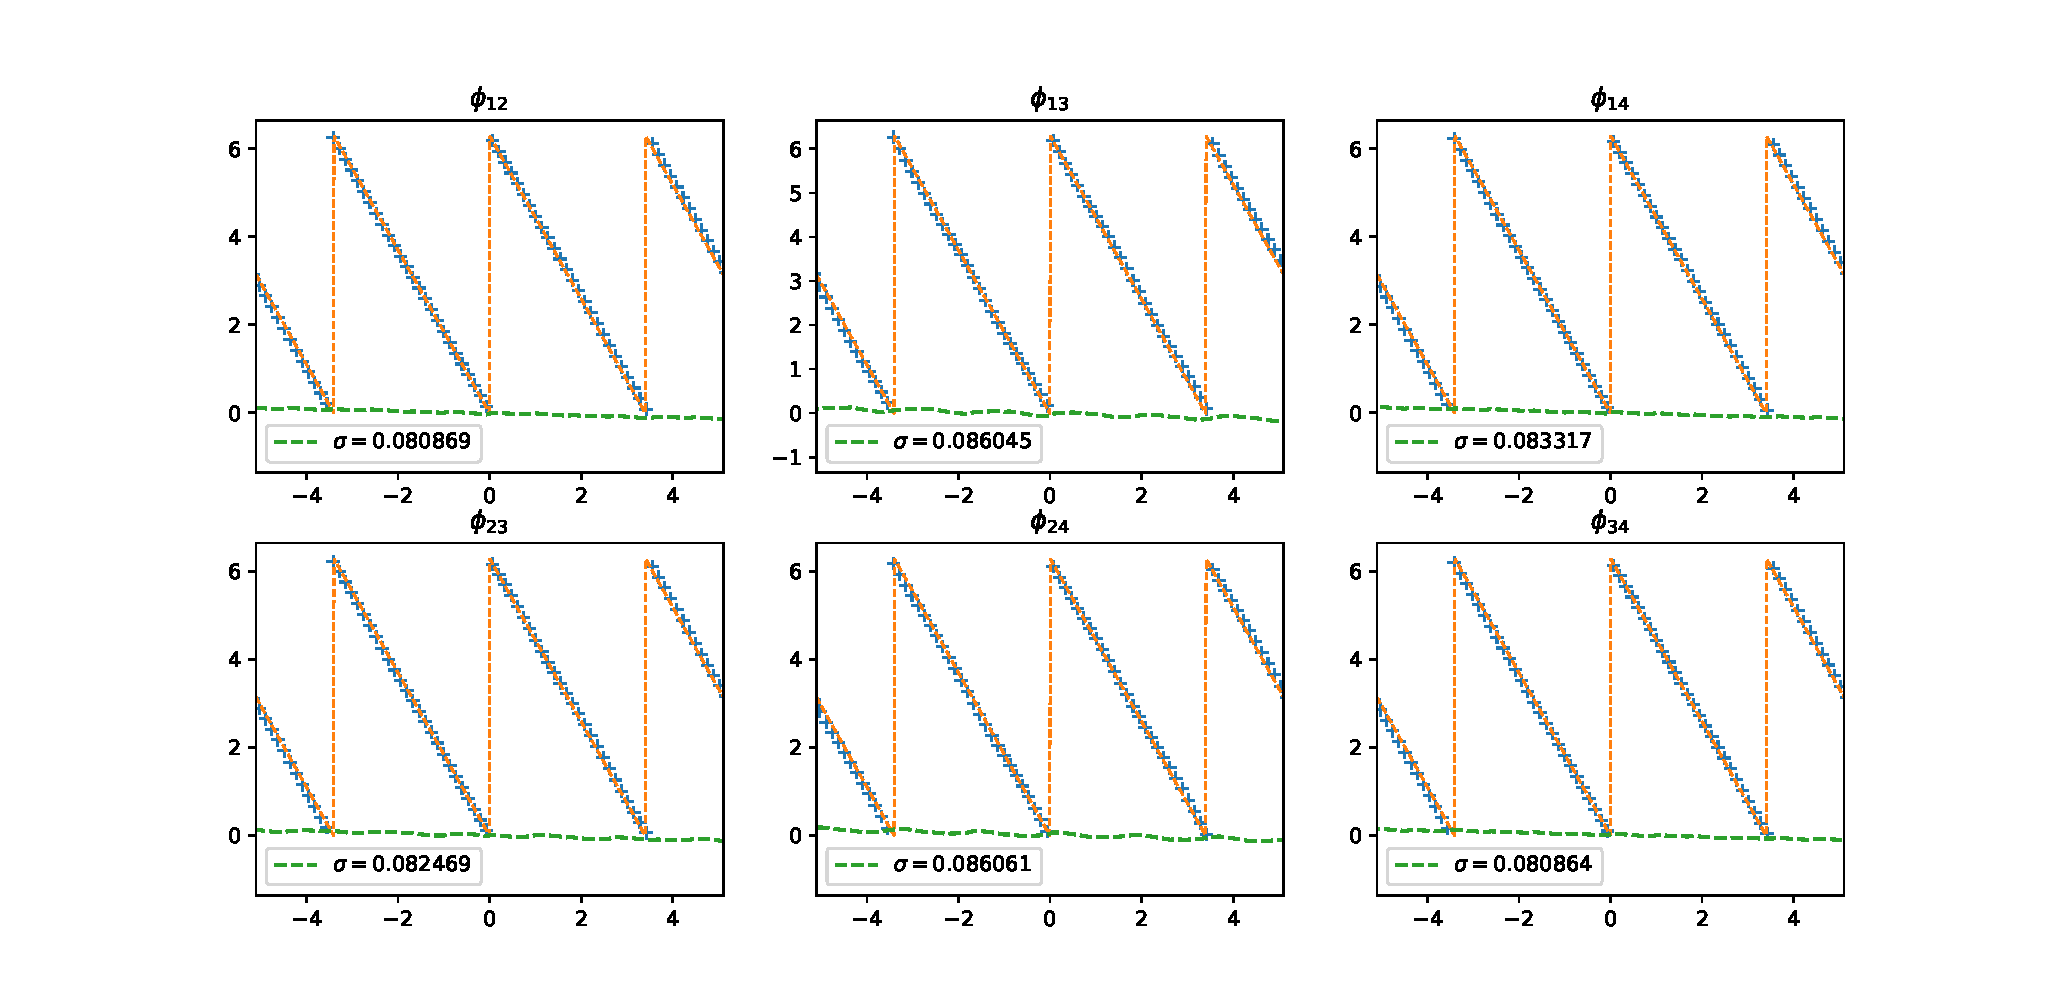
\includegraphics[scale=.4]{../picture/retrieve_phase_simu.pdf}
     \caption{The simulated retrieved phases of the optimised component at $\lambda=3.4\si{\micro\meter}$ and bandwidth=70nm. The x-axis is the OPD in µm and the y-axis the phase in rad. Baseline numbering follows the ones from Fig.\ref{fig:retrieved_phase_expe}.The blue line is the actual retrieved data the orange line the theoretical result and the green line the residues (difference between the blue and orange one). $\sigma$ is the standard deviation to 0 of the residues in rad.}
     \label{an:retrieved_phase_simu}
    \end{figure}

\newpage
\printglossary

\newpage
\bibliographystyle{alpha}
\bibliography{biblio}

\end{document}    
